\begin{mdframed}[style=warning]
	\begin{ejercicio}
		\textbf{Conceptos.}
		\begin{enumerate}
			\item Si las cargas circulan muy lentamente a través de un metal, ¿por qué no es necesario que pasen horas para que se encienda una luz cuando usted activa el interruptor?
			\item Un estudiante afirma que el segundo de dos focos en serie es menos brillante que el priemro, ya que éste consume parte de la corriente. ¿Qué respondería a esta afirmación?
		\end{enumerate}
	\end{ejercicio}
\end{mdframed}






\begin{mdframed}[style=warning]
	\begin{ejercicio}
		Una envolvente esférica, con radio interior $r_a$ y radio exterior $r_b$, ser forma a partir de un material de resistividad $\rho$. Porta corriente radialmente, con densidad uniforme en todas direcciones. Encuentre la resistencia.
	\end{ejercicio}
\end{mdframed}





\begin{mdframed}[style=warning]
	\begin{ejercicio}
		Un material de resistividad $\rho$ se modela como un cono truncado de altura $h$. El extremo inferior tiene un radio $b$, en tanto que el extremo $a$. Suponga que la corriente está uniformemente distribuida en cualquier sección transversal circular del cono, de forma que la densidad de la corriente no dependerá de la posición radial. (La densidad de corriente variará dependiendo de su posición a lo largo del eje del cono.) Encuentre la resistencia.
	\end{ejercicio}
\end{mdframed}






\begin{mdframed}[style=warning]
	\begin{ejercicio}
		Como se muestra en la figura, una red de resistores de resistencias $R_1$ y $R_2$ se extiende infinitamente hacia la derecha. Demuestre que la ressitencia total $R_T$ de la red infinita es igual a
			$$ R_T = R_1 + \sqrt{R_1 ^2 + 2R_1 R_2}. $$
			
		\begin{figure}[H]
			\centering
			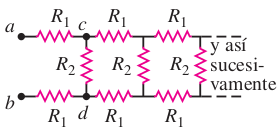
\includegraphics[scale=0.5]{./img/redinfinita.png}
			\caption{Red Infinita}
			\label{Red}
		\end{figure}
	\end{ejercicio}
\end{mdframed}






\begin{mdframed}[style=warning]
	\begin{ejercicio}
		Para no perder la costumbre. Considere que un resistor $R$ está a lo largo de cada arista de un cubo con conexiones en las esquinas. Encuentre la resistencia equivalente entre dos esquinas del cubo diagonalmente opuestas.
		\begin{figure}[H]
			\centering
			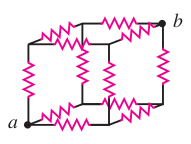
\includegraphics[scale=0.5]{./img/cubito.png}
			\caption{Cubo de resistencias}
			\label{cubito}
		\end{figure}
	\end{ejercicio}
\end{mdframed}







\begin{mdframed}[style=warning]
	\begin{ejercicio}
		Encuentre las corrientes $I_1$, $I_2$ y $I_3$ mostradas en la figura.
		\begin{figure}[H]
			\centering
			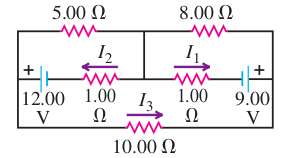
\includegraphics[scale=0.5]{./img/circ.png}
			\caption{Circuito.}
			\label{circ}
		\end{figure}
	\end{ejercicio}
\end{mdframed}


















































%%%